\documentclass{article}

\usepackage[utf8]{inputenc}
\usepackage[spanish]{babel}

\usepackage{geometry}               % Márgenes del documento
\usepackage{amsfonts}
\usepackage{graphicx}

\usepackage[nottoc]{tocbibind}

\usepackage{color}
\usepackage[pdftex, colorlinks=true, linkcolor=blue, urlcolor=red, filecolor=magenta, citecolor=blue]{hyperref}
\definecolor{gray97}{gray}{.97}
\definecolor{gray75}{gray}{.75}
\definecolor{gray45}{gray}{.45}

\usepackage{listings}
\usepackage[usenames,dvipsnames]{xcolor}
\colorlet{keyword}{blue!100!black!80}
\colorlet{STD}{Lavender}
\colorlet{comment}{green!80!black!90}

\lstset{ %
	backgroundcolor=\color{white},
	breaklines=true,
	numbers=left,
	numbersep=5pt,
	numberstyle=\tiny\color{gray45}
}

\lstdefinestyle{instance}{
	language     = bash,
	tabsize=3,
	numbers=left, % Donde se situan los numeros
	frame=none, % Se pone un marco
	showstringspaces=false, % No muestre el cuadrado en los espacios de los strings
	backgroundcolor = \color{gray75},
	basicstyle   = \footnotesize \ttfamily,
	keywordstyle = [1]\color{keyword}\bfseries,
	keywordstyle = [2]\color{STD}\bfseries,
	breaklines=true,                % sets automatic line breaking
	commentstyle = \color{comment}
}


\geometry{a4paper}                  % Tamaño y márgenes del documento
\geometry{left=2.5cm,top=2.5cm}
\geometry{bottom=2.5cm,right=2.5cm}

\geometry{driver=dvips,pdftex} % ???
\setcounter{secnumdepth}{5}    % ???
\setcounter{tocdepth}{5}       % ???

\setlength{\parskip}{\baselineskip} % Espacio entre párrafos (una linea en blanco)

%--------------------------------------------------------------------------
\title{\textbf{Plataforma como Servicio}
\\ \textbf{\emph{Servicios móviles de Amazon Web Services}}
}
\author{Francisco Abel Cedrón Santaeufemia \and \textit{francisco.cedron@udc.es}}
\date{} %Asi no inserta la fecha

\addto\captionsspanish{
\def\tablename{Tabla}
\def\listtablename{Índice de tablas}
}

\begin{document}
\maketitle % Pone titulo, autor
\renewcommand{\abstractname}{Abstract} % El nombre que aparece al principio del abstract
\begin{abstract}
En este documento se explicará el uso de varios servicios que ofrece \emph{Amazon Web Services} en la categoría de plataforma como servicio centrándonos en la parte de dispositivos móviles. Aunque el SDK para móviles de \emph{Amazon Web Services} proporciona acceso optimizados para servicios como \emph{Amazon S3}, \emph{Amazon DynamoDB}, \emph{Amazon SQS} o \emph{Amazon Kinesis} entre otros, en este trabajo sólo se hablará de los servicios \emph{Amazon Cognito}, \emph{Amazon Mobile Analytics} y \emph{Amazon SNS Mobile Push} que son los tres servicios que ofrece \emph{Amazon Web Services} exclusivamente para el uso de dispositivos móviles.
\end{abstract}
\renewcommand{\contentsname}{} % Lo que pone en el indice
{\setlength{\parskip}{0mm} \tableofcontents} % Para que no ponga espacios entre las lineas de indice
%\vspace{1cm} % Para dejar un espacio con respecto a la tabla

\newpage

\section{Introducción}
	Un hecho innegable de la época actual es que gracias a los smartphones ha cambiado la manera de usar las nuevas tecnologías hasta tal punto que existen ciertos estudios de mercado que indican que el uso de ordenadores personales se irán sustituyendo por el uso de dispositivos móviles como pueden ser las tablets o los smartphones.

	El aumento de uso de los dispositivos móviles se debe en su mayor medida a la gran variedad de aplicaciones que se pueden ejecutar en ellos. El uso de las aplicaciones para móviles es tan importante que algunas empresas se preocupan más de actualizar su versión para los dispositivos móviles que en su versión para el ordenador. Un ejemplo de ello es \emph{Telegram}, donde su versión para ordenador está en la revisión 1.32 para \emph{Mac OS X}\footnote{
Telegram para Mac OS X	\url{https://itunes.apple.com/us/app/messenger-for-telegram/id747648890}}
y en la 0.6.14 para \emph{Windows}\footnote{
Telegram para Windows \url{https://tdesktop.com/}}, 
mientras que las versiones para móviles están en las versiones 2.0.4, 2.7.2 y 1.1.3.46 para \emph{Android}\footnote{
Telegram para Android \url{https://play.google.com/store/apps/details?id=org.telegram.messenger}}
, \emph{iOS}\footnote{
Telegram para iOS \url{https://itunes.apple.com/app/telegram-messenger/id686449807}}
y \emph{Windows Phone}\footnote{
Telegram para Windows Phone

\url{http://www.windowsphone.com/en-us/store/app/telegram-messenger-beta/945b96a7-aadc-4dd0-806a-c2d1e0e6ca9a}}
respectivamente.

	Debido a la importancia que exigen los usuarios a la calidad en las aplicaciones cada vez más desarrolladores están empleando servicios usados en la nube para poder ofrecer un mejor servicio.
	
	En este trabajo nos centraremos en algunas de las soluciones que ofrece Amazon Web Services dentro de la categoría de Plataforma como Servicio. Entre ellas nos centraremos en el uso de \emph{Amazon Cognito}\cite{Cognito} cuyo uso es para la gestión de identidades y sincronización, \emph{Amazon Mobile Analytics}\cite{Analytics} que se emplea es el análisis de datos de uso de las aplicaciones y \emph{Amazon SNS Mobile Push}\cite{Sns} para el envío de notificaciones.

%%Hay que decir en algun sitio que:
%%Los servicios para móviles de AWS se pueden utilizar en todas las plataformas y están diseñados para ayudar a crear aplicaciones en plataformas iOS, Android y Fire OS.

\section{Amazon Cognito}

	\emph{Amazon Cognito}  es uno de los servicios que ofrece \emph{Amazon Web Services} diseñado especialmente para dispositivos móviles. \emph{Amazon Cognito} es un servicio para almacenar los datos de usuario como las preferencias de las aplicaciones o el estado de los juegos en la nube de AWS. Con este servicio, es posible guardar los datos de las aplicaciones localmente en los dispositivos de los usuarios, lo que permite que las aplicaciones funcionen incluso aunque los dispositivos no estén conectados a internet. La ventaja de este servicio es que el desarrollador pueda centrarse en el funcionamiento de la aplicación para ofrecer una buena experiencia de uso en lugar de preocuparse por desarrollar y gestionar una solución de backend para la gestión de identidades, el estado de la red, el almacenamiento y la sincronización.

\subsection{Beneficios de usar \emph{Amazon Cognito}}

\subsubsection{Gestión de identidad}
	\emph{Amazon Cognito} es un servicio para la identifiación de usuarios que puede mantener sincronizados los datos de los usuarios entre distintos dispositivos. Para la identificación de usuarios permite usar proveedores de inicio de sesión público como Amazon, Google y Facebook.  Además permite guardar los datos de las aplicaciones localmente, lo que supone que los usuarios puedan usar las aplicaciones sin estar conectados a internet.
	
	Una de las ventajas que permite es que los usuarios empiecen a probar las aplicaciones en modo invitado de tal manera que los usuarios pueden empezar a probar la aplicación sin autenticarse, pero si más adelante el usuario quiere autenticarse puede hacerlo con uno de los proveedores de inicio de sesión público compatibles permitiendo que el usuario conserve sus datos. 
	
%	Aunque \emph{Amazon Cognito} está especialmente diseñado para desarrolladores de aplicaciones móviles a través de un SDK también expone una API de servidor con lo que se puede emplear este servicio sin la restricción de que la aplicación sea tenga que ser exclusivamente para un dispositivo móvil.
	
	Además \emph{Amazon Cognito} no recibe ni almacena las credenciales de los usuarios. Al comunicarse directamente con un proveedor de identidad público sólo se guarda el token recibido por el proveedor de tal manera que no recibe ninguna información confidencial como podría ser el correo electrónico. Además esto permite una autenticación federada, almacenamiento de de los datos de perfil en un almacén de sincronización y distribución de tokens de acceso de \emph{Amazon Web Services} sin necesidad de escribir unos sistemas propios de autenticación e identidad en el backend.

	\emph{Amazon Cognito} admite la existencia de diferentes identidades en un mismo dispositivo. Como cada identidad se gestiona por separado, el desarrollador puede escoger la manera en la que la aplicación inicia y cierra las sesiones de los usuarios y la manera en la que se almacenan los datos remotos y locales de la aplicación.

	Una de las ventajas que promueve \emph{Amazon} es que este servicio es la creación de un conjunto de identidades de tal manera que \emph{Amazon Cognito} ofrece un contenedor donde guardar de manera ordenada las identidades de los usuarios finales de las aplicaciones. El desarrollador puede asociar un mismo conjunto de identidades con una sola aplicación o con varias. Si utiliza dos conjuntos de identidades diferentes para dos aplicaciones, el mismo usuario final dispondrá de un identificador exclusivo distinto en cada una de las aplicaciones.

\subsubsection{Almacenamiento de los datos de la aplicación}

	\emph{Amazon Cognito} provee un almacén de sincronización que no es más que un lugar donde guardar los datos en forma de pares \emph{clave,valor} vinculados a una identidad. Cada identidad incluida en el almacén de sincronización dispone de su propio almacén de información de usuario, además no impone ninguna restricción respecto al número de identidades que se pueden crear en los conjuntos de identidades. 
	
	Cada almacén de datos de información de usuario puede tener un tamaño máximo de 20 MB. Cada conjunto de datos incluido en un almacén de información de usuario puede contener hasta 1MB de datos. En cada conjunto de datos puede haber hasta 1024 claves. Tanto las claves como los valores almacenados en los conjuntos de datos son cadenas alfanuméricas, no existiendo limitación de la longitud (siempre y cuando no supere la limitación de 1MB). Según \emph{Amazon} está limitación de 1MB en los conjuntos de datos es para que la acción de sincronización se ejecute correctamente sin tener que realizar varios intentos aunque el ancho de banda del usuario sea limitado.
	
	Los datos no se guardan directamente en el almacén de sincronización, los datos se guardan en una base de datos SQLite en el dispositivo local, de tal manera que la aplicación pueda acceder a ellos en cualquier momento. Los datos se envían al almacén de sincronización llamando a un método específico que realiza la sincronización. 

\subsubsection{Sincronización de los datos}

	Para la sincronización de datos, el método que realiza la sincronización  lee la versión más reciente de los datos disponible en el almacén de sincronización de \emph{Amazon Cognito} y la compara con la copia local guardada en caché. Después de realizar la comparación, si es necesario, el método de sincronización escribe las actualizaciones en el almacén de sincronización de \emph{Amazon Cognito} y en el almacén local. De manera predeterminada se conserva la versión más reciente de los datos, pero el desarrollador puede cambiar este configuración y obtener ambas versiones de los datos. De esta forma, se le permite al desarrollador decidir que versión de lo datos, si la que está en el almacén de sincronización o la copia local, desea conservar.

\subsection{Precios}

	El precio se basa en la cantidad total de datos que estén en el almacén de sincronización y la cantidad de veces que se usan las operaciones de sincronización \footnote{
La comparación de la copia local del dispositivo con el almacén de sincronización y la sincronización de datos son consideradas operaciones de sincronización}
. La autenticación de los usuarios y la generación de identificadores no son consideradas operaciones de sincronización y  de momento son gratuitas sin importar el número de veces que se realicen.

	Los costes de \emph{Amazon Cognito} son \textit{0,15 USD} por 10000 operaciones de sincronización y \textit{0,15 USD} por GB de capacidad en el almacén de sincronización que además se facturan por mes.
	
\begin{table}[h]
	\begin{center}
		\caption{Ejemplo de costes con \emph{Amazon Cognito}.}
		\begin{tabular}{|l|c|r|}
\cline{2-3}
\multicolumn{1}{c|}{}
& \textbf{Uso} & \multicolumn{1}{|c|}{\textbf{Coste}} \\ \hline
\hline
\textit{Operaciones de sincronización} & 1000000 & (1000000/10000) x 0,15 = \textit{15,00 USD} \\ \hline
\textit{Espacio del almacén de sincronización} & 4,77 GB & 4,77 x 0,15 = \textit{0,72 USD} \\ \hline
\hline
\textit{\color{red}Total} & \multicolumn{2}{|r|}{ \textit{\color{red} 15,72 USD}} \\ \hline
		\end{tabular}
		\label{tab:PrizeAmazonCognito}
	\end{center}
\end{table}

\section{Amazon Mobile Analytics}

\subsection{Aspectos generales}

	\emph{Amazon Mobile Analytics} es uno de los servicios que ofrece \emph{Amazon Web Services} diseñado especialmente para dispositivos móviles. \emph{Amazon Mobile Analytics} es un servicio que permite almacenar, visualizar y comprender los datos de uso de las aplicaciones.
	
%http://blog.woorank.com/2014/08/20-mobile-analytics-tools-for-mobile-website-and-apps/
	Muchas soluciones para el análisis de aplicaciones móviles ofrecen los datos de uso después que hayan pasado varias horas, mientras que \emph{Amazon Mobile Analytics} se ha diseñado para tener listos los informes de uso pasados los 60 minutos después de la recepción de los datos desde una aplicación.
	Por ejemplo, con \emph{Google Analytics} las actualizaciones son cada 4 horas o cada 24 según la cuenta premiun o estándar \cite{GoogleAnalytics}. \emph{Flurry Analytics} se actualiza después de unas horas aunque no especifica cada cuánto tiempo\cite{FlurryAnalytics}, aunque hay usuarios que indican que algunos eventos se muestran pasados unos minutos, algunas métricas pueden llegar a tardar varias horas \footnote{\url{http://stackoverflow.com/questions/9545456/flurry-analytics-basic-analytics-issues} (dentro de la página de stackoverflow hay un email con la respuesta de support)}. \emph{Apsalar}, otra herramienta de análisis, indica que algunos datos se actualizan al momento, pero otros pueden llegar a tardar aproximadamente un día \cite{Apsalar}.

\subsection{Informes de \emph{Amazon Mobile Analytics}}

	Amazon nos proporciona dos maneras de obtener la información que se ha guardado usando \emph{Amazon Mobile Analytics}, mediante su consola web\footnote{AWS Management Console \url{https://console.aws.amazon.com/mobileanalytics/home/}} (ver la figura \ref{fig:Overview}), o descargando los datos en archivos CSV (ver la figura \ref{fig:CSV}).

\begin{figure}[h]
  \centering
    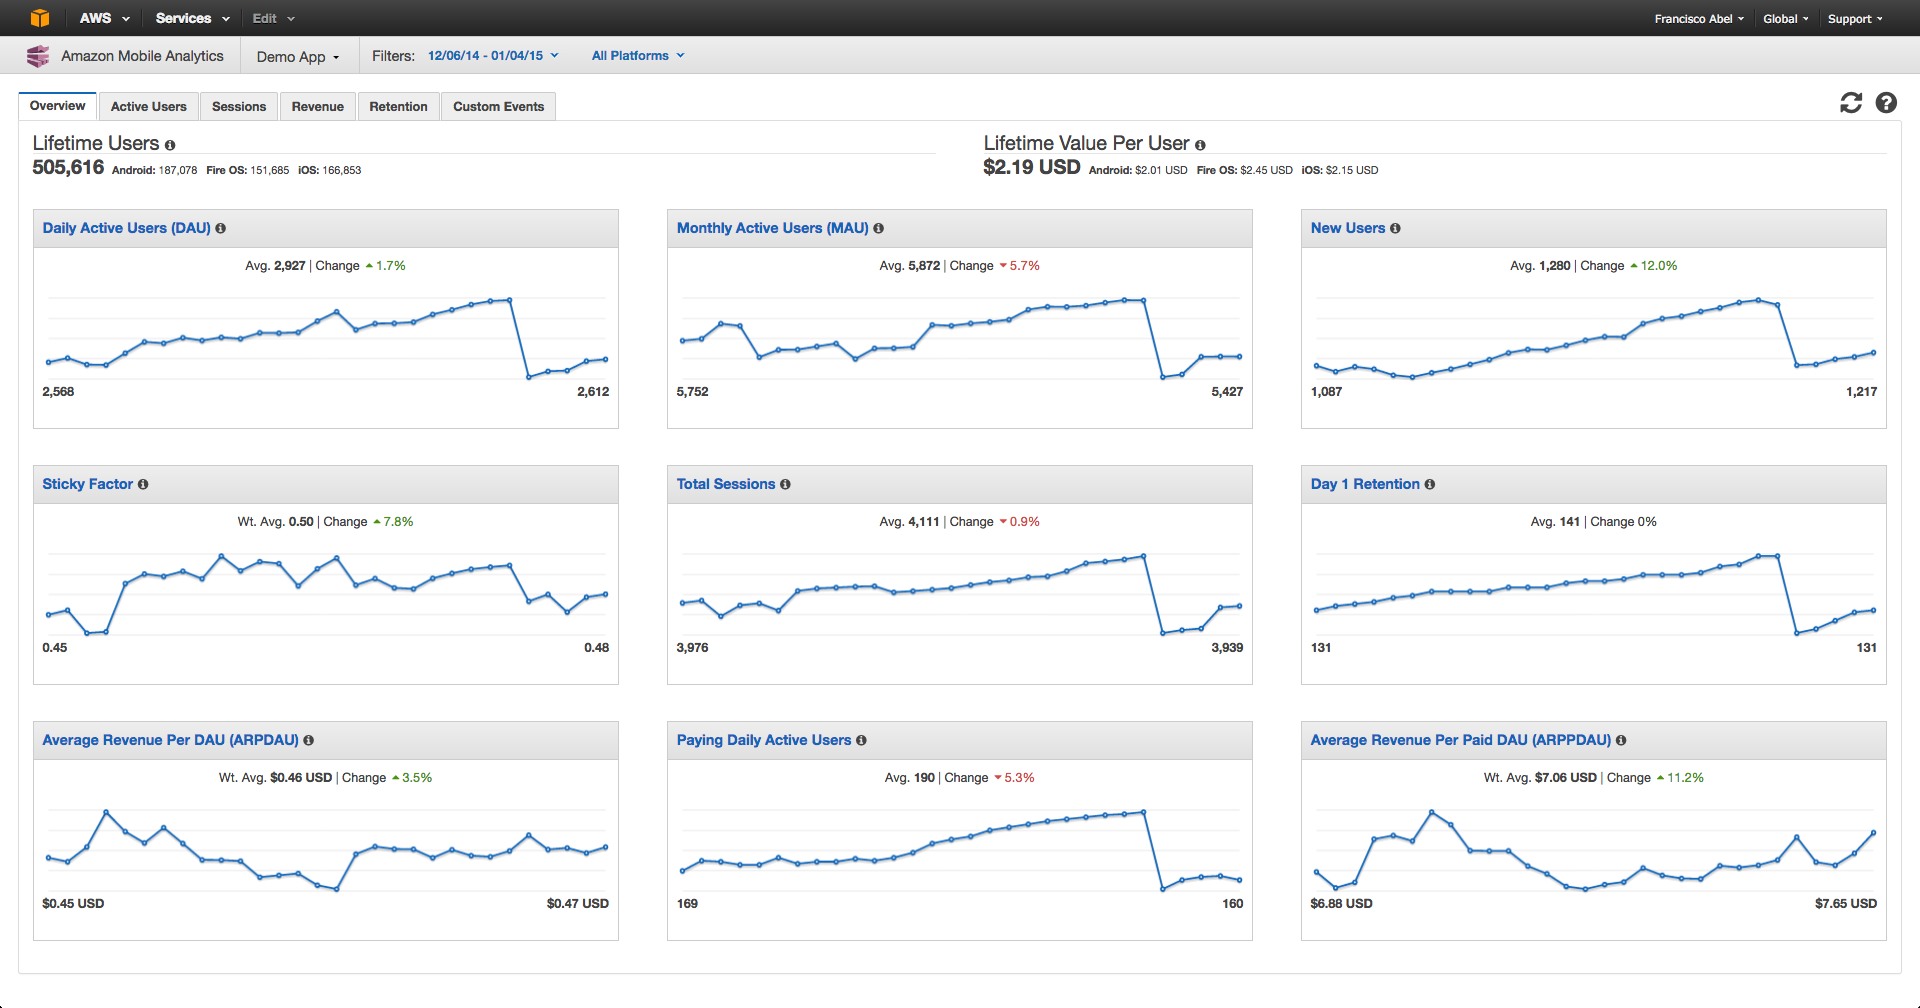
\includegraphics[width=0.9\textwidth]{img/001_Overview.png}
  \caption{Informe en AWS  Management Console.}
  \label{fig:Overview}
\end{figure}

\begin{figure}[h]
\centering
\lstinputlisting{files/Demo.csv}
\caption{Fichero en formato CSV de usuarios activos .}
\label{fig:CSV}
\end{figure}

	Las métricas que podemos consultar son las siguientes:
\begin{itemize}
	\item \textbf{Usuarios activos} (véase la figura \ref{fig:ActiveUsers})
	\begin{itemize}
		\item \textbf{Usuarios activos diarios} (DAU, Daily Active Users).
		\item \textbf{Usuarios activos mensuales} (MAU, Monthly Active Users).
		\item \textbf{Nuevos usuarios} (New Users)
		\item \textbf{Factor de ``pegajosidad''} (Sticky Factor): Es un factor para indicar lo enganchados que están los usuarios a la aplicación (DAU dividido entre MAU).
	\end{itemize}
	\item \textbf{Sesiones} (véase la figura \ref{fig:Sessions})
	\begin{itemize}
		\item \textbf{Sesiones totales} (Total Sessions): número de veces que se utilizó la aplicación en un día concreto.
		\item \textbf{Promedio de sesiones por usuario} (Average Number of Sessions Per Daily Active User)
	\end{itemize}
	\item \textbf{Ingresos} (véase la figura \ref{fig:Revenue})
	\begin{itemize}
		\item \textbf{Usuarios activos diarios que pagan} (Paying Daily Active Users)
		\item \textbf{Ingresos medios por usuario activo diario} (ARPDAU, Average Revenue Per Daily Active User)
		\item \textbf{Ingresos medios por usuario activo diario pagado} (ARPPDAU, Average Revenue Per Paid Daily Active User)
		\item \textbf{Usuarios activos mensuales que pagan} (Paying Monthly Active Users)
		\item \textbf{Ingresos medios por usuario activo mensual} (ARPMAU, Average Revenue Per Monthly Active User)
		\item \textbf{Ingresos medios pos usuario activo mensual pagado} (ARPPMAU, Average Revenue Per Paid Monthly Active User)
	\end{itemize}
	\item \textbf{Retención} (véase la figura \ref{fig:Retention})
	\begin{itemize}
		\item \textbf{Retención diaria}: Incluye la retención de 1, 3  y 7 días para nuevos usuarios
		\item \textbf{Retención semanal}: Incluye la retención de 1, 2 y 3 semanas para nuevos usuarios.
	\end{itemize}
	\item \textbf{Eventos personalizados}: Eventos específicos para la aplicación que se pueden definir como cuando un usuario alcanza en un juego el final de un nivel
\end{itemize}

	Para poder usar \emph{Amazon Mobile Analytics} hay que tener una forma de identificación en \emph{Amazon Web Services} para lo cual, podemos hacerlo de dos maneras distintas:
{\setlength{\parskip}{0mm} 
\begin{itemize}
	\item Con \emph{Amazon Cognito}
	\item Con \emph{AWS Identity and Access Managment} \cite{IAM}.
\end{itemize}
}

	Como todos los servicios de \emph{Amazon Web Services} para dispositivos móviles, se puede emplear \emph{Amazon Mobile Analytics} para los sistemas iOS, Android y Fire OS, además de que permite mostrar los informes separando por plataformas, como se muestra en la figura \ref{fig:OverviewIOS}, de tal manera que los desarrolladores se puedan centrar más en un sistema según los resultados que se obtengan.
	
	Además, cabe mencionar unos detalles importantes del funcionamiento de esta tecnología:
{\setlength{\parskip}{0mm} 
\begin{itemize}
	\item Como los usuarios de las aplicaciones pueden estar en distintas franjas horarias los informes se muestran en UTC.
	\item Esta tecnología sólo está disponible en la región este de EE.UU. (Norte de Virginia).
	\item La forma de enviar los eventos es por lotes y se envían cada minuto (en el caso de que exista eventos a enviar). 
	\item Se puede especificar el transporte para enviar los eventos:
	\begin{enumerate}
		\item WiFi y Datos.
		\item Sólo WiFi.
	\end{enumerate}
\end{itemize}
}

\begin{figure}[h]
  \centering
    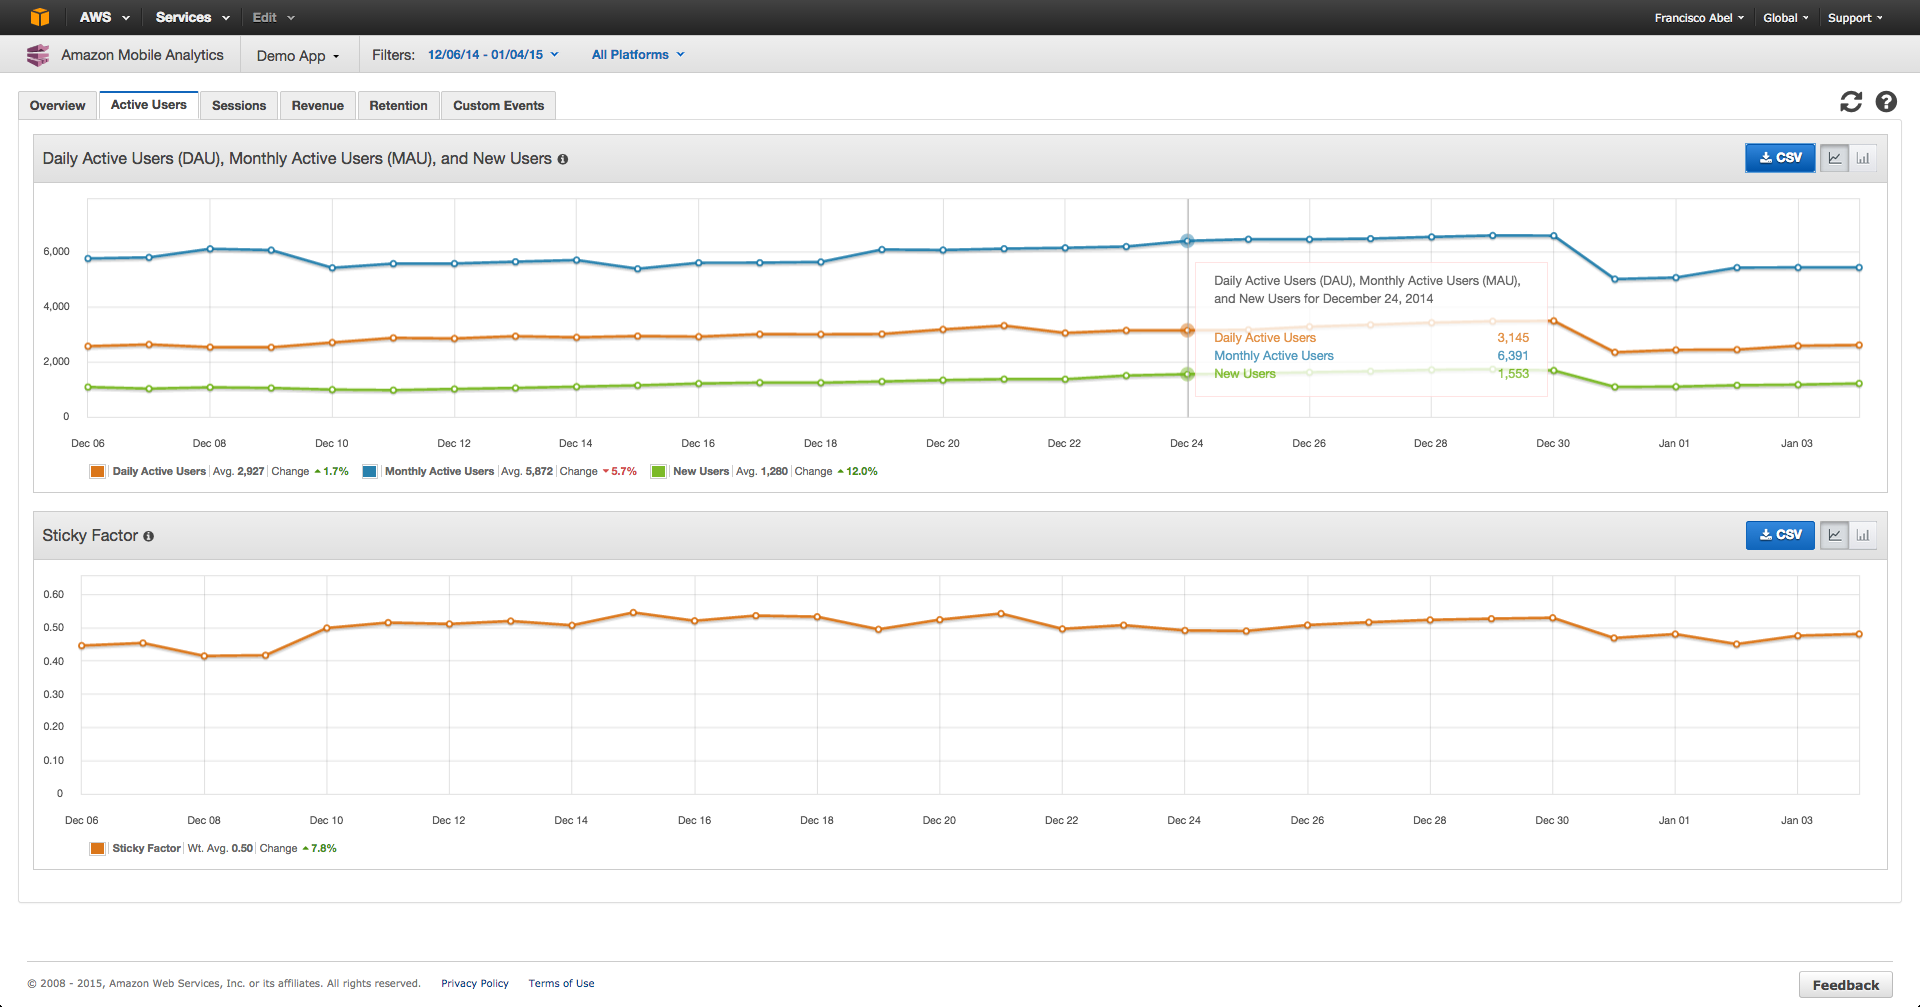
\includegraphics[width=0.9\textwidth]{img/002_Active_Users.png}
  \caption{Informe de usuarios activos mostrado en AWS  Management Console.}
  \label{fig:ActiveUsers}
\end{figure}

\begin{figure}[h]
  \centering
    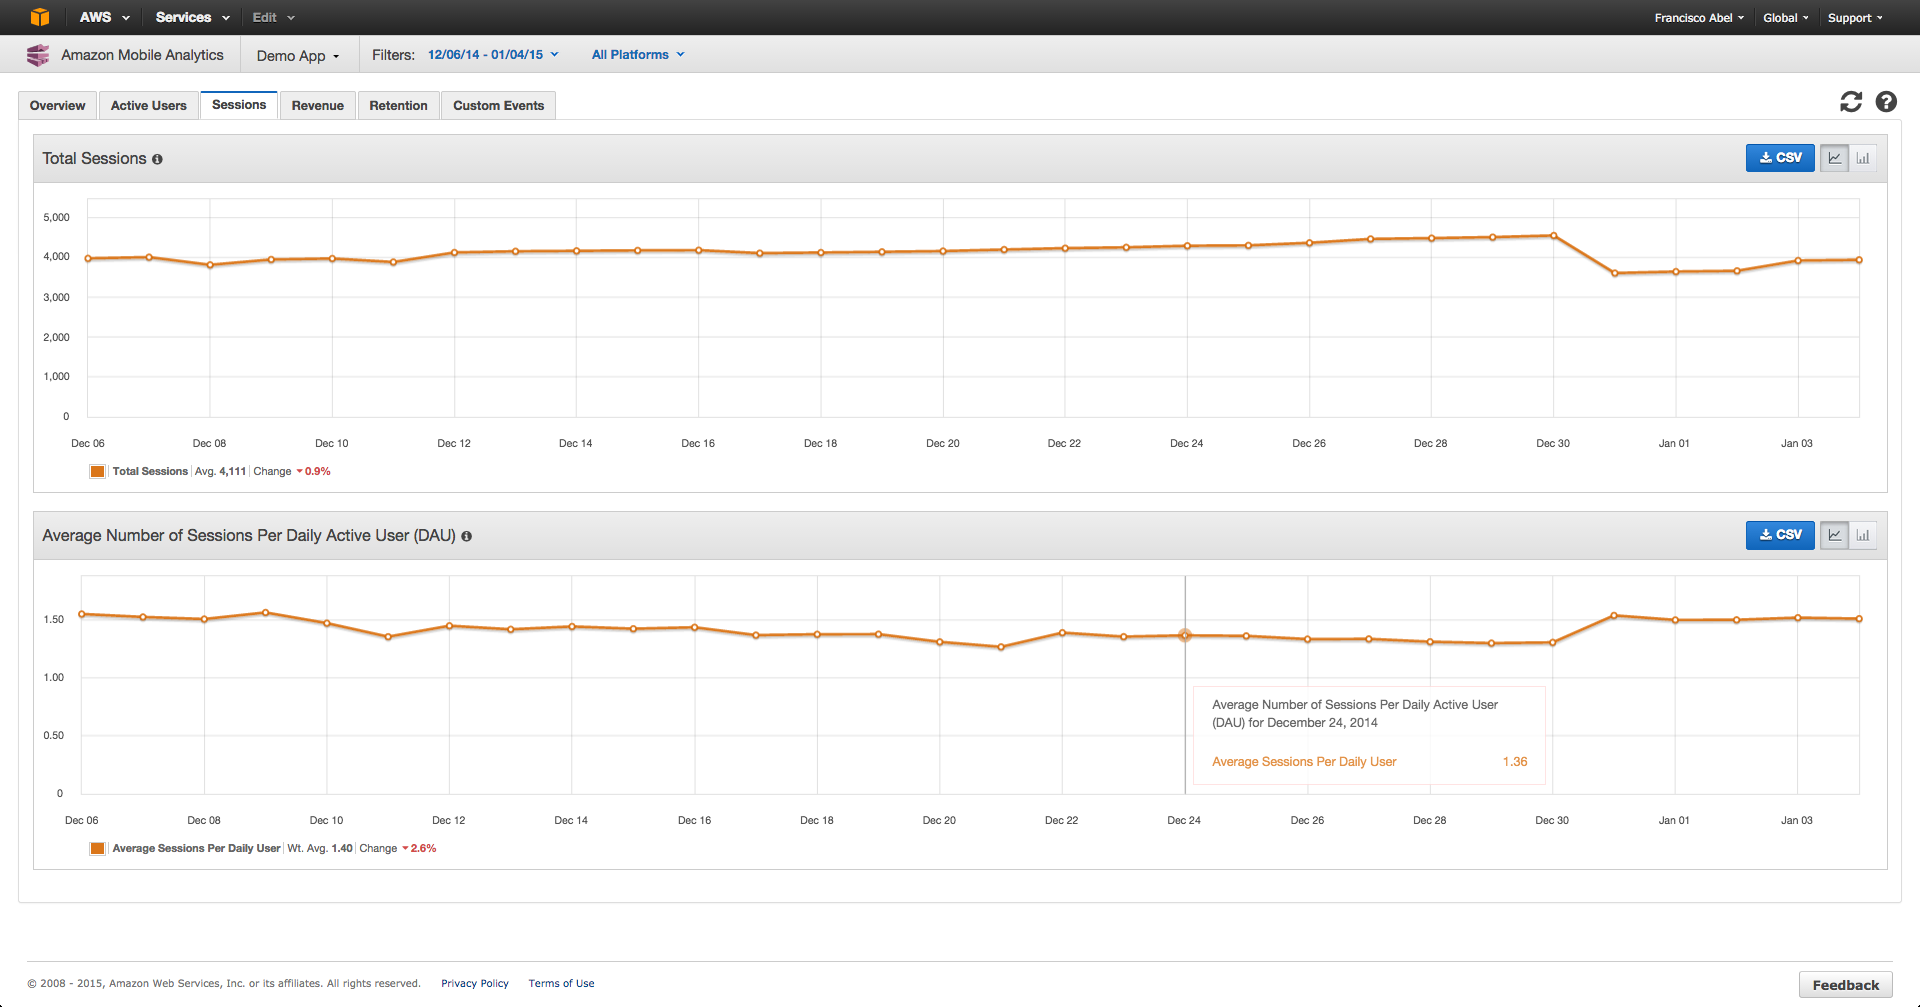
\includegraphics[width=0.9\textwidth]{img/003_Sessions.png}
  \caption{Informe de sesiones mostrado en AWS  Management Console.}
  \label{fig:Sessions}
\end{figure}

\begin{figure}[h]
  \centering
    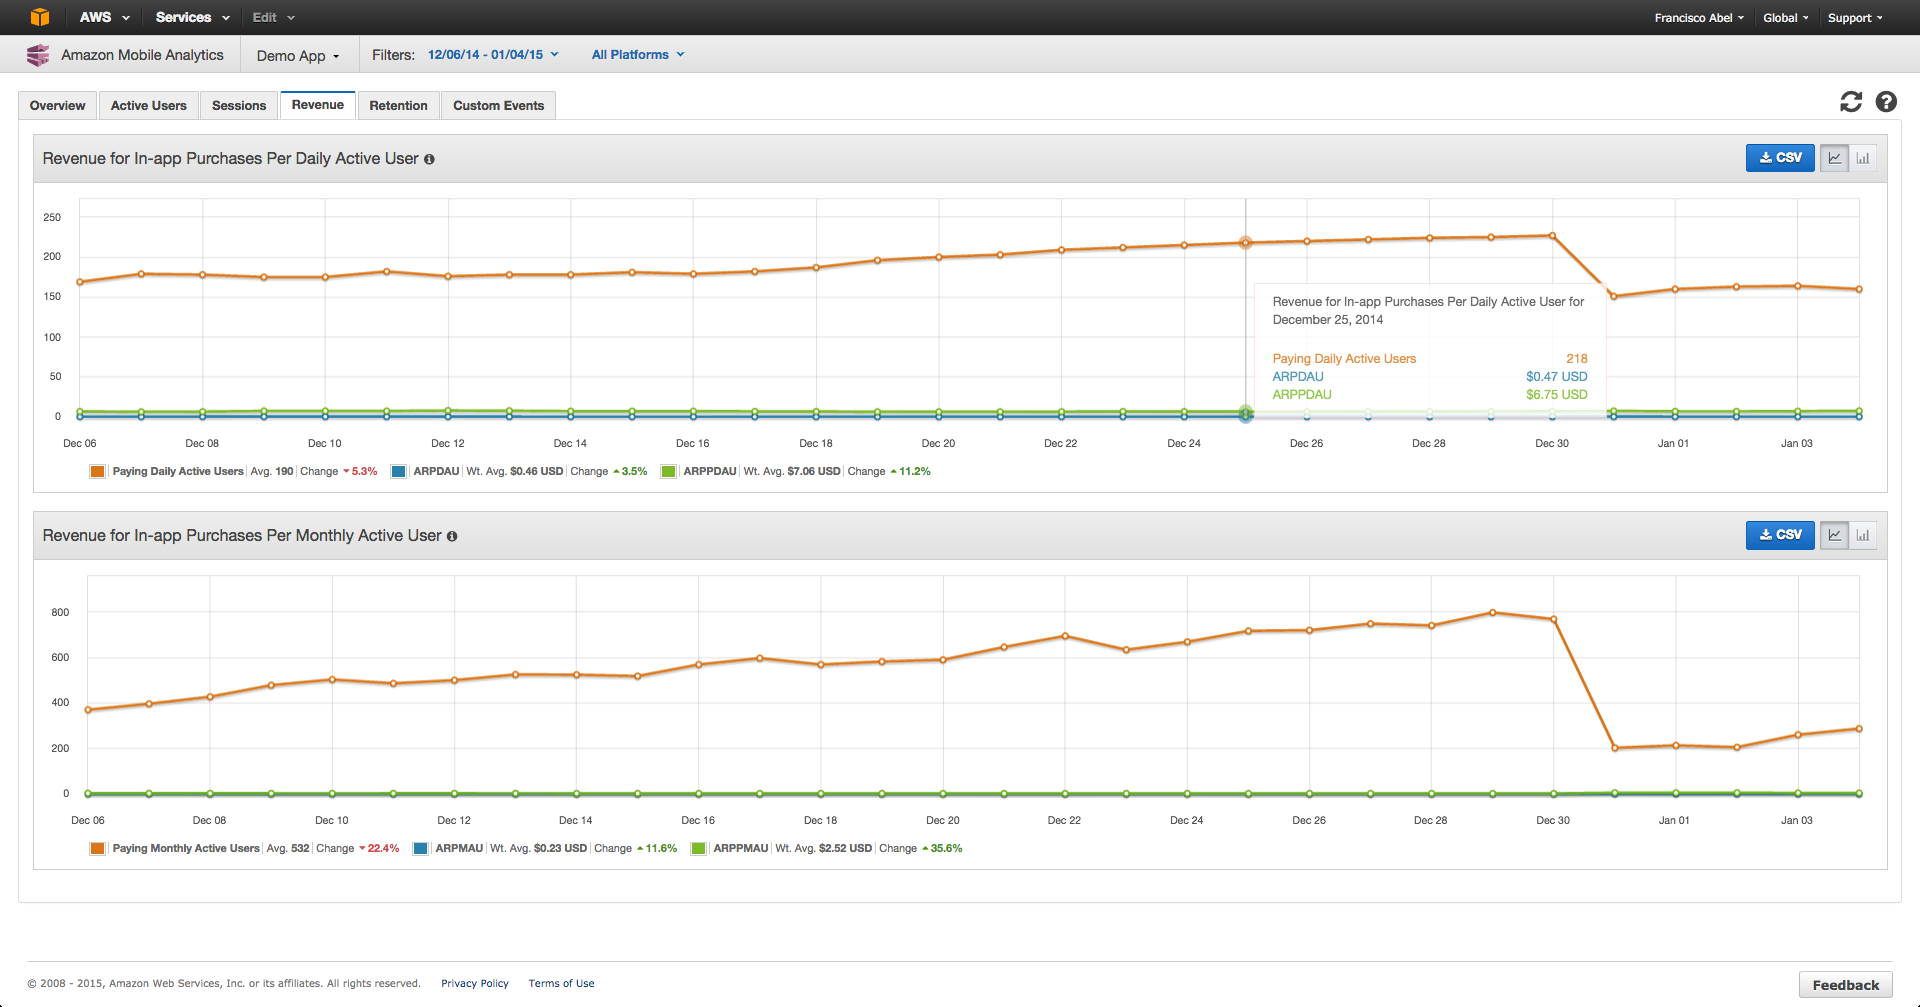
\includegraphics[width=0.9\textwidth]{img/004_Revenue.png}
  \caption{Informe de ingresos mostrado en AWS  Management Console.}
  \label{fig:Revenue}
\end{figure}

\begin{figure}[h]
  \centering
    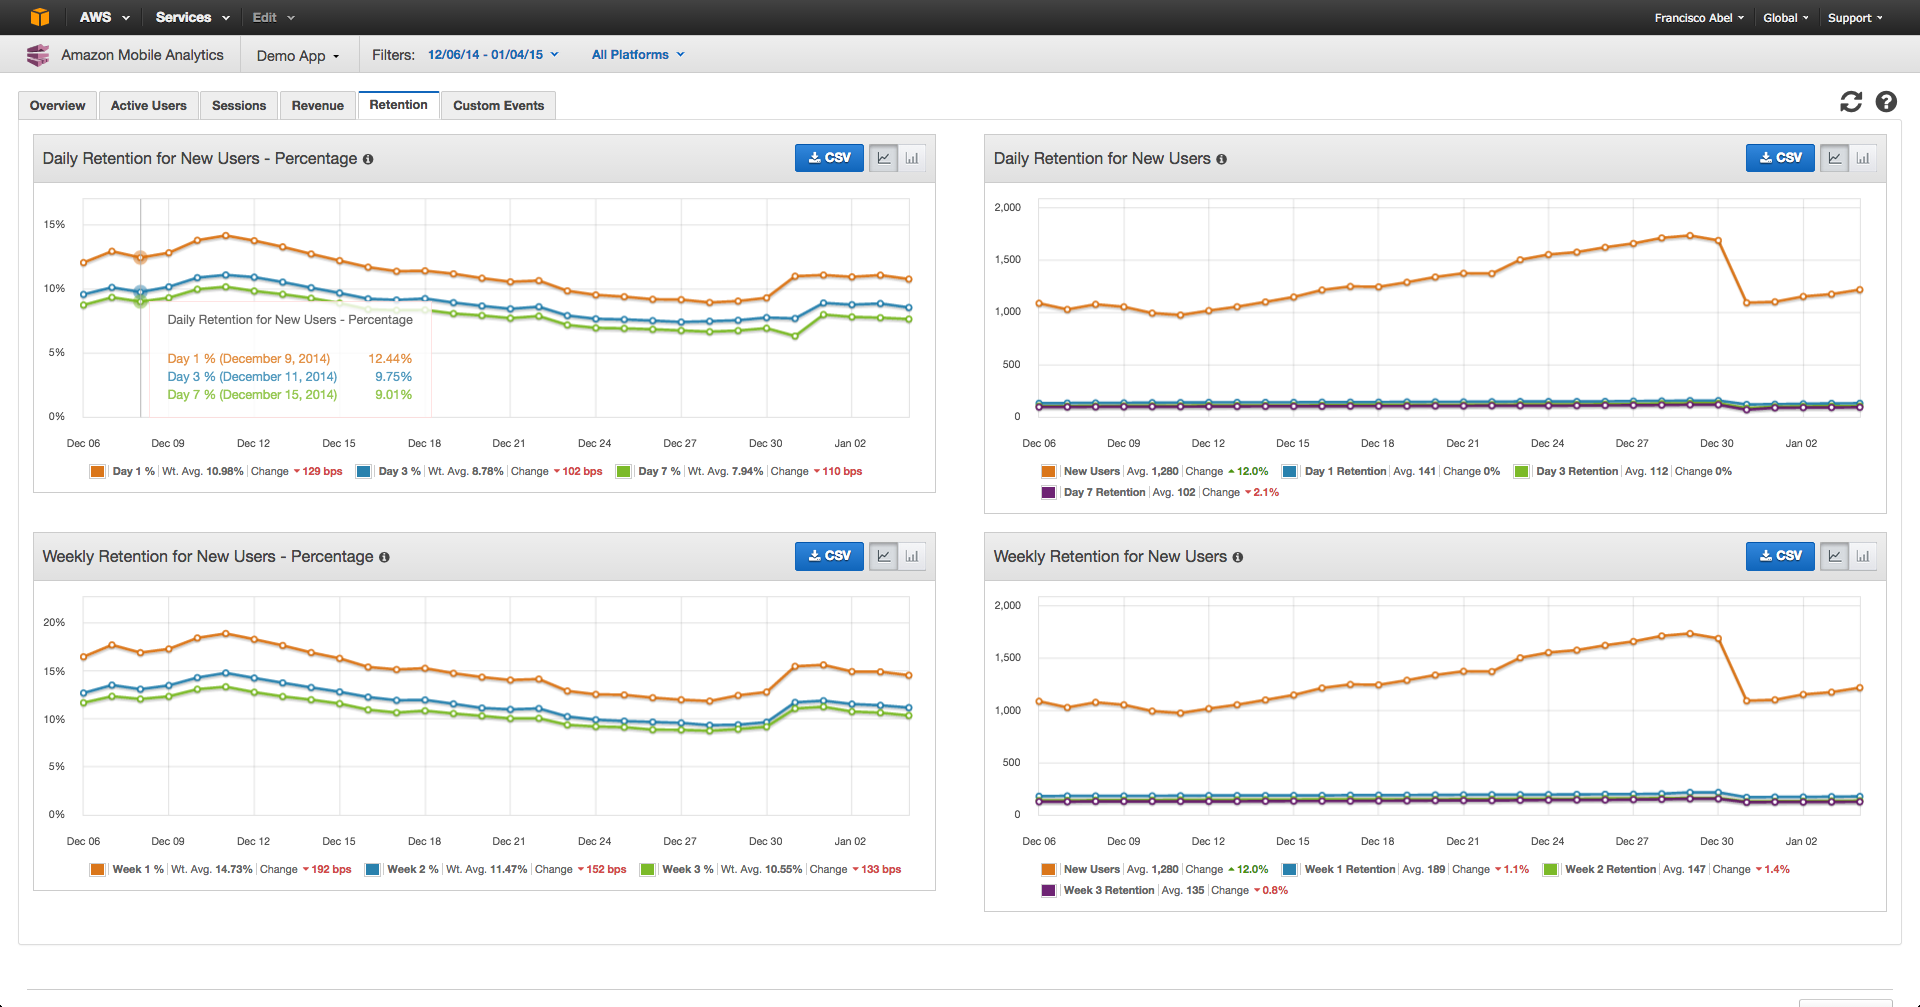
\includegraphics[width=0.9\textwidth]{img/005_Retention.png}
  \caption{Informe de retención mostrado en AWS  Management Console.}
  \label{fig:Retention}
\end{figure}


\begin{figure}[h]
  \centering
    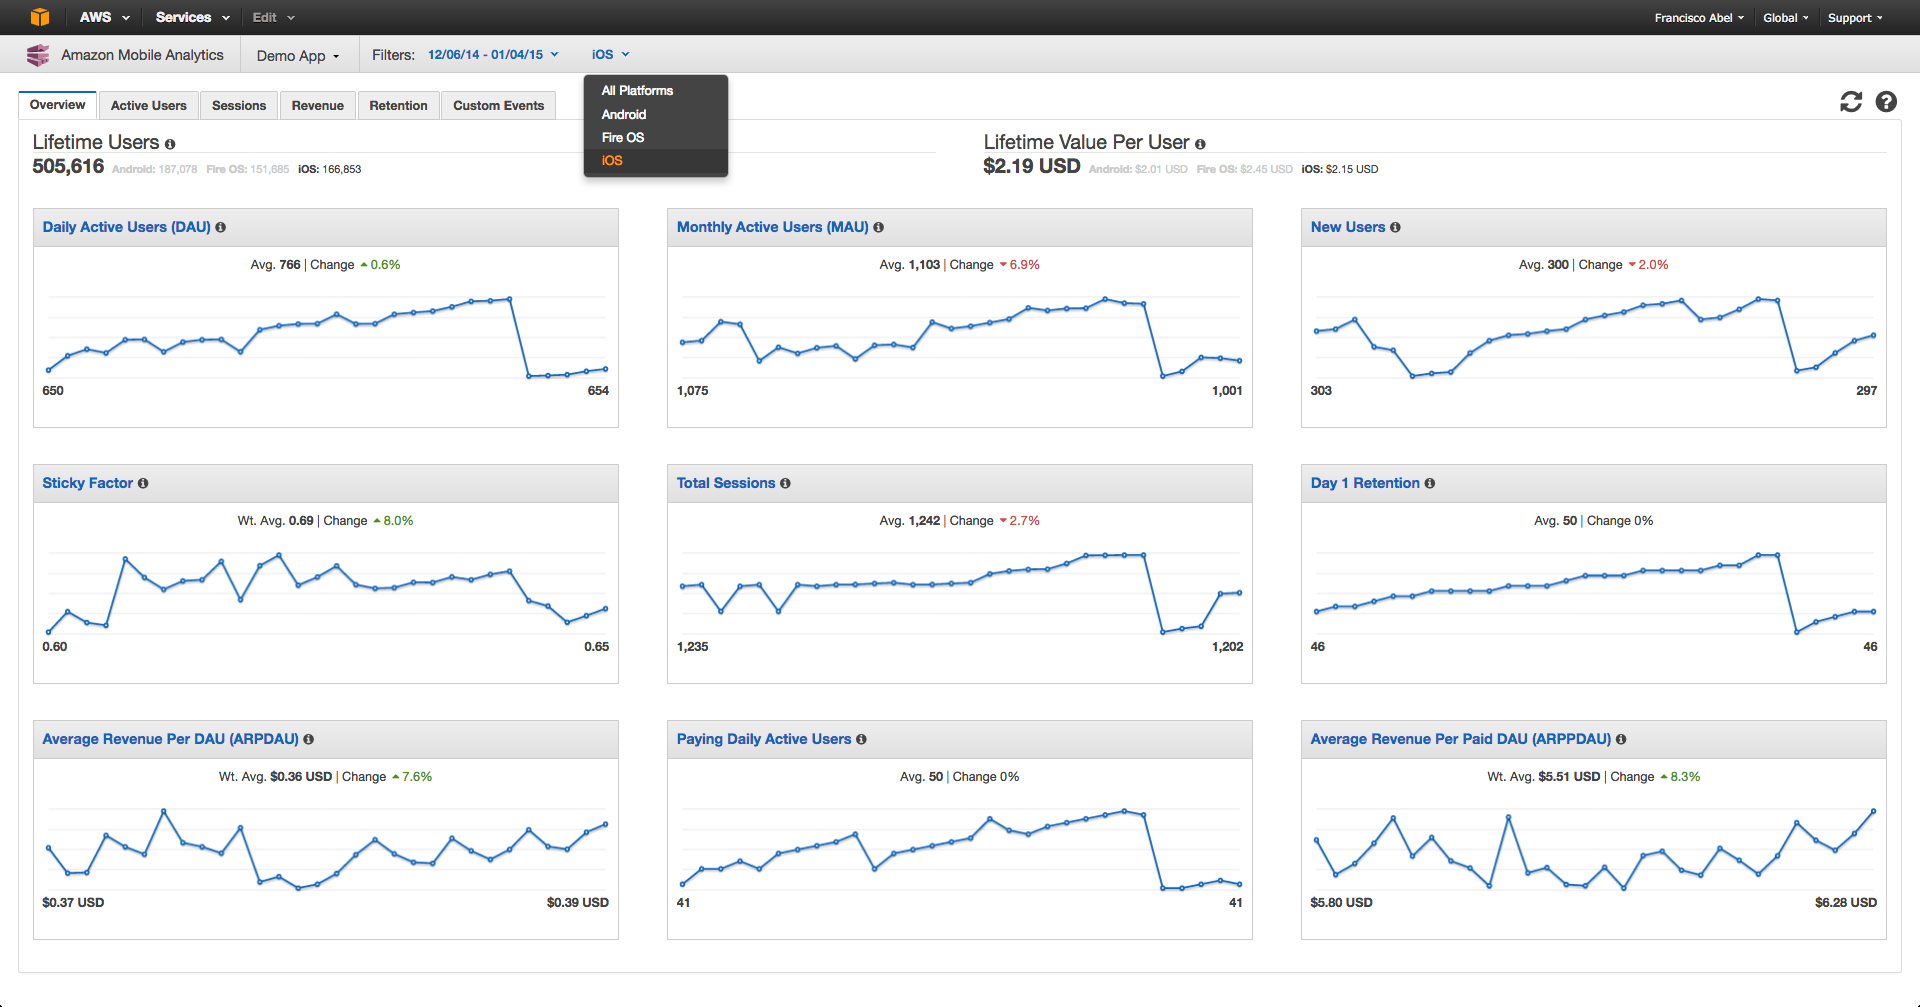
\includegraphics[width=0.9\textwidth]{img/006_iOS.png}
  \caption{Informe mostrado en AWS  Management Console para dispositivos iOS.}
  \label{fig:OverviewIOS}
\end{figure}

\clearpage

\subsection{Precios}
	El servicio ofrece un capa gratuita de 100 millones de eventos al mes, después el precio de \emph{Amazon Mobile Analytics} es de \textit{1 USD} por cada millón de eventos al mes. Existen tres tipos de eventos:
\begin{itemize}
{\setlength{\parskip}{0mm} 
	\item \textbf{Eventos del sistema} como puede ser el inicio o el fin de una sesión
	\item \textbf{Eventos de compras realizadas desde la aplicación}
	\item \textbf{Eventos personalizado}s como por podría ser que un usuario complete un nivel en un juego	
}
\end{itemize}

	Cuando se utiliza el SDK para móviles de AWS, por cada sesión de la aplicación envía 2 eventos del sistema (para poder indicar el principio y el fin de una sesión). Después el resto de eventos se generan en base a las comprar que se realicen o al número de eventos personalizados que se han generado.

\begin{table}[h]
	\begin{center}
		\caption{Ejemplo de costes con \emph{Amazon Mobile Analytics}.}
		\begin{tabular}{|l|p{5cm}|}
\hline
\textbf{Sesiones mensuales} & 20 millones \\ \hline
\textbf{Eventos procesados por sesión} & 2 eventos de sistema por sesión y 10 eventos personalizados por sesión. \textit{(12 Eventos por sesión)}\\ \hline
\textbf{Eventos procesados en total} & 12 * 20 millones = \textit{240 millones de eventos} \\ \hline
\textbf{\color{red} Coste} & (240 - 100) x 1 = \textit{\color{red} 140 USD} \\ \hline
		\end{tabular}
		\label{tab:PrizeAmazonMobileAnalytics}
	\end{center}
\end{table}

\section{Amazon SNS Mobile Push}

\subsection{Aspectos generales}
	Antes de empezar a hablar de \emph{Amazon SNS Mobile Push} hay que indicar que es el único de los tres servicios para dispositivos móviles que se encuentra en fase beta.
	
	\emph{Amazon Simple Notification Service Mobile Push} es un servicio de mensajería para enviar mensajes de tipo push a dispositivos móviles con iOS, Android, Fire OS, así como a toros servicios distribuidos.
	
	Además de enviar notificaciones en la nube directamente a los dispositivos, el servicio puede enviar notificaciones mediantes mensajes SMS o correo electrónico, así como a las colas de \emph{Amazon Simple Queue Service}\cite{SQS}.

\subsection{Características de \emph{Amazon SNS Mobile Push}}
	\emph{Amazon SNS Mobile Push} permite enviar mensajes push a dispositivos móviles o servicios distribuidos. Con este servicio se puede optar por enviar mensajes exclusivos a determinados dispositivos de Apple, Google o Amazon, o bien difundir los mensajes a multitud de dispositivos móviles con una única solicitud de publicación.
	
	Cuando se empieza a usar este servicio, lo primero a crear es un tema que realiza las funciones de ``punto de acceso'' (que es el que identifica un asunto o tipo de evento concreto) para la publicación de mensajes y permitir que los clientes se suscriban a las notificaciones. En cuanto se crea un tema, el propietario del tema puede definir políticas, como limitar quién puede publicar mensajes o suscribirse a notificaciones, o especificar que protocolos de notificación serán compatibles (como, por ejemplo, SMS, correo electrónico...). Los suscriptores son usuarios interesados en recibir notificaciones de temas de interés; pueden suscribirse a un tema o su propietario puede suscribirlos. Los que especifican el protocolo y el extremo son los suscriptores. Cuando los publicadores tienen información o actualizaciones para avisar a los suscriptores pueden publicar un mensaje en el tema (lo que hará que \emph{Amazon SNS} distribuya el mensaje a todos los suscriptores).
	
	Además \emph{Amazon SNS} es compatible con \emph{AWS CloudTrail}\cite{CloudTrail} lo que permite obtener un historial de información, como la identidad de la persona que ha efectuado la llamada a la API, la hora de la llamada, la dirección IP de dicha persona, los parámetros de solicitud y los elementos de respuesta enviados por \emph{Amazon SNS}.
	
	A día de hoy, \emph{Amazon SNS} funciona con otros servicios de \emph{Amazon Web Services} como \emph{Amazon Simple Queue Service} y \emph{Elastic Compute Cloud (EC2)}\cite{EC2}. Por ejemplo, las aplicaciones que se encuentren en ejecución en \emph{EC2} podrán publicar información en \emph{Amazon SNS}, y que estas se transladen a los usuarios u otras aplicaciones.

\subsubsection{Formato de distribución para las notificaciones}
	\emph{Amazon SNS} ofrece una amplia flexibilidad para la entrega de notificaciones donde los usuarios son quienes especifican el mecanismo de transporte a la hora de suscribirse a un tema. Los protocolos de transporte son:
{\setlength{\parskip}{0mm} 
\begin{itemize}
	\item \textit{Notificaciones push a móbiles}
	\item \textit{HTTP/HTTPS}: Los suscriptores especifican una URL como parte del registro de suscripción, donde las notificaciones se enviarán a través de una petición POST a dicha URL
	\item \textit{Email/Email-JSON}: Los mensajes se envián a las direcciones registradas en forma de correo electrónico. \textit{Email-JSON} envía las notificaciones como objeto JSON, mienstra que \textit{Email} envía correos electrónicos basados en texto
	\item \textit{Simple Queue Service}: Los susaruios pueden especificar una cola donde \emph{Amazon SNS} colocará el mensaje de notificación
	\item \textit{SMS}\footnote{Actualmente sólo admite números de teléfono de EE.UU.} Mensaje de texto que se envía al número de teléfono registrado
\end{itemize}
}	

\subsubsection{Plataformas de notificaciones push}
Actualmente se admiten las siguientes plataformas de notificaciones push:
{\setlength{\parskip}{0mm} 
\begin{itemize}
	\item \emph{Amazon Device Messaging (ADM)}
	\item \emph{Apple Push Notification Service (APNS)}
	\item \emph{Google Cloud Messaging (GCM)}
	\item Servicio de notificaciones push de Windows \emph{(WNS)} para \emph{Windows 8+} y \emph{Windows 8.1+}
	\item Servicio de notificaciones push de Microsoft \emph{MPNS} para \emph{Windows Phone 7+}
	\item \emph{Baidu Cloud Push} para dispositivos \emph{Android} en China
\end{itemize}
}

\subsubsection{Operaciones disponibles}

	\emph{Amazon SNS} ofrece diversas API para crear notificaciones de eventos para los propietarios de temas, suscriptores y publicadores.
{\setlength{\parskip}{0mm} 
\begin{itemize}
	\item {Operaciones del propietario}
	\begin{itemize}
		\item \textit{CreateTopic}: Crear un nuevo tema
		\item \textit{DeleteTopic}: Eliminar un tema anteriormente creado
		\item \textit{ListTopics}: Lista de temas de los que es propietario un usuario
		\item \textit{ListSubscriptionsByTopic}: Lista de suscripciones de un tema determinado
		\item \textit{SetTopicAttributes}: Establecer o modificar los atributos de un tema, como la modificación de permisos del publicador o suscriptor, los métodos de transporte...
		\item \textit{GetTopicAttributes}: Obtener los atributos existentes de un tema determinado
		\item \textit{AddPermission}: otorgar acceso a los usuarios para acciones especificadas
		\item \textit{RemovePermission}: eliminar permisos para acciones especificadas a usuarios determinados.
	\end{itemize}
	\item {Operaciones del suscriptor}
	\begin{itemize}
		\item \textit{Subscribe}: Registrar una nueva suscripción sobre un tema determinado.
		\item \textit{ConfirmSubscription}: Responder a un mensaje de confirmación de suscripción
		\item \textit{UnSubscribe}: Cancelar una suscripción de un tema
		\item \textit{ListSubscriptions}: Listar las suscripciones propiedad de un determinado usuario
	\end{itemize}
	\item {Operaciones del publicador}
	\begin{itemize}
		\item \textit{Publish}: Publicar un nuevo mensaje en un tema
	\end{itemize}
\end{itemize}
}

	
\subsection{Precios}
	Los precios de entrega varían en función del tipo de extremo (véase la tabla \ref{tab:PrizeSNS}).
	
	Actualmente, \emph{Amazon SNS} permite un límite máximo de 256KB para los mensajes publicados. Además cada porción de 64KB de datos publicados se factura como una solicitud. Por ejemplo, una sola llamada a API con una carga de 256KB se factura como cuatro solicitudes.
	
\begin{table}[h]
	\begin{center}
		\caption{Ejemplo de costes con \emph{Amazon SNS Mobile Push}.}
		\begin{tabular}{|l|c|}
\hline
\textbf{Tipo de extremo} & \textbf{Precio} \\ \hline
Notificaciones push a móviles & 0,50 USD por millón \\ \hline
SMS & 0,15 por 100 \\ \hline
Correo electrónico & 2,00 USD por 100000 \\ \hline
HTTP/s & 0,60 por millón \\ \hline
\emph{Simple Queue Service (SQS)} & Las entregas a colas de \emph{SQS}  se realizan sin cargos \\ \hline
		\end{tabular}
		\label{tab:PrizeSNS}
	\end{center}
\end{table}



\clearpage
{\setlength{\parskip}{0mm} \listoffigures} % Para que no ponga espacios entre las lineas de indice

{\setlength{\parskip}{0mm} \listoftables}

% Bibliografía.
%-----------------------------------------------------------------
\clearpage

\renewcommand{\bibname}{Referencias}
\begin{thebibliography}{99}
\bibitem{Cognito}
Documentacion de \emph{Amazon Cognito}

\url{http://aws.amazon.com/es/documentation/cognito/}
\bibitem{Analytics}
Documentación de \emph{Amazon Mobile Analytics}

\url{http://docs.aws.amazon.com/mobileanalytics/latest/ug/welcome.html}
\bibitem{Sns}
Documentación de \emph{Amazon SNS Mobile Push}

\url{http://docs.aws.amazon.com/sns/latest/dg/SNSMobilePush.html}
\bibitem{GoogleAnalytics}
Características de \emph{Google Analytics}

\url{http://www.google.com/intl/es/analytics/premium/features.html}
\bibitem{FlurryAnalytics}
Soporte de \emph{Flurry Analytics}

\url{http://support.flurry.com/index.php?title=Analytics/FAQ#Where.E2.80.99s_my_data.3F_How_often_is_data_updated_on_the_Flurry_portal.3F}

\url{http://support.flurry.com/index.php?title=Publisher/FAQ#How_often_is_reporting_updated.3F}
\bibitem{Apsalar}
Soporte de \emph{Apsalar}

\url{http://support.apsalar.com/customer/portal/questions/1157971-how-long-does-it-take-approximately-for-analytics-data-to-show-up-in-your-account-}
\bibitem{IAM}
Documentación de \emph{AWS Identity and Access Managment}

\url{http://docs.aws.amazon.com/IAM/latest/UserGuide/IAM_Introduction.html}
\bibitem{SQS}
Documentación de \emph{Amazon Simple Queue Service}

\url{http://docs.aws.amazon.com/AWSSimpleQueueService/latest/SQSGettingStartedGuide/Welcome.html}
\bibitem{EC2}
Documentación de \emph{Amazon Compute Cloud}

\url{http://docs.aws.amazon.com/AWSEC2/latest/UserGuide/concepts.html}
\bibitem{CloudTrail}
Documentación de \emph{AWS CloudTrail}

\url{http://docs.aws.amazon.com/awscloudtrail/latest/userguide/what_is_cloud_trail_top_level.html}

\end{thebibliography}

\end{document}
